
\subsection{Description of DNA Mismatch Repair}

%In \cite{10.1007/978-3-319-99498-7_8} a DNA repair mechanism was modelled using CCB. The problem to deal with was the incorporation into DNA of a base which should not occur in DNA at all. The repair relied on recognizing this base. Another possible error is that two bases are included which are both possible in DNA, but do not match, for example, a pair of adenine and cytosine. This can happen if, after the splitting of the double strand, the new strand intended to match the old one, does not actually match the old strand - for example, incorporating an adenine opposite a cytosine, which should normally be matched by a thymine. Figure~\ref{fig:damages} shows such a mismatch in the upper right position: The combination of the A/G bases is incorrect.

%\begin{figure}[h!]
%  \centering
%    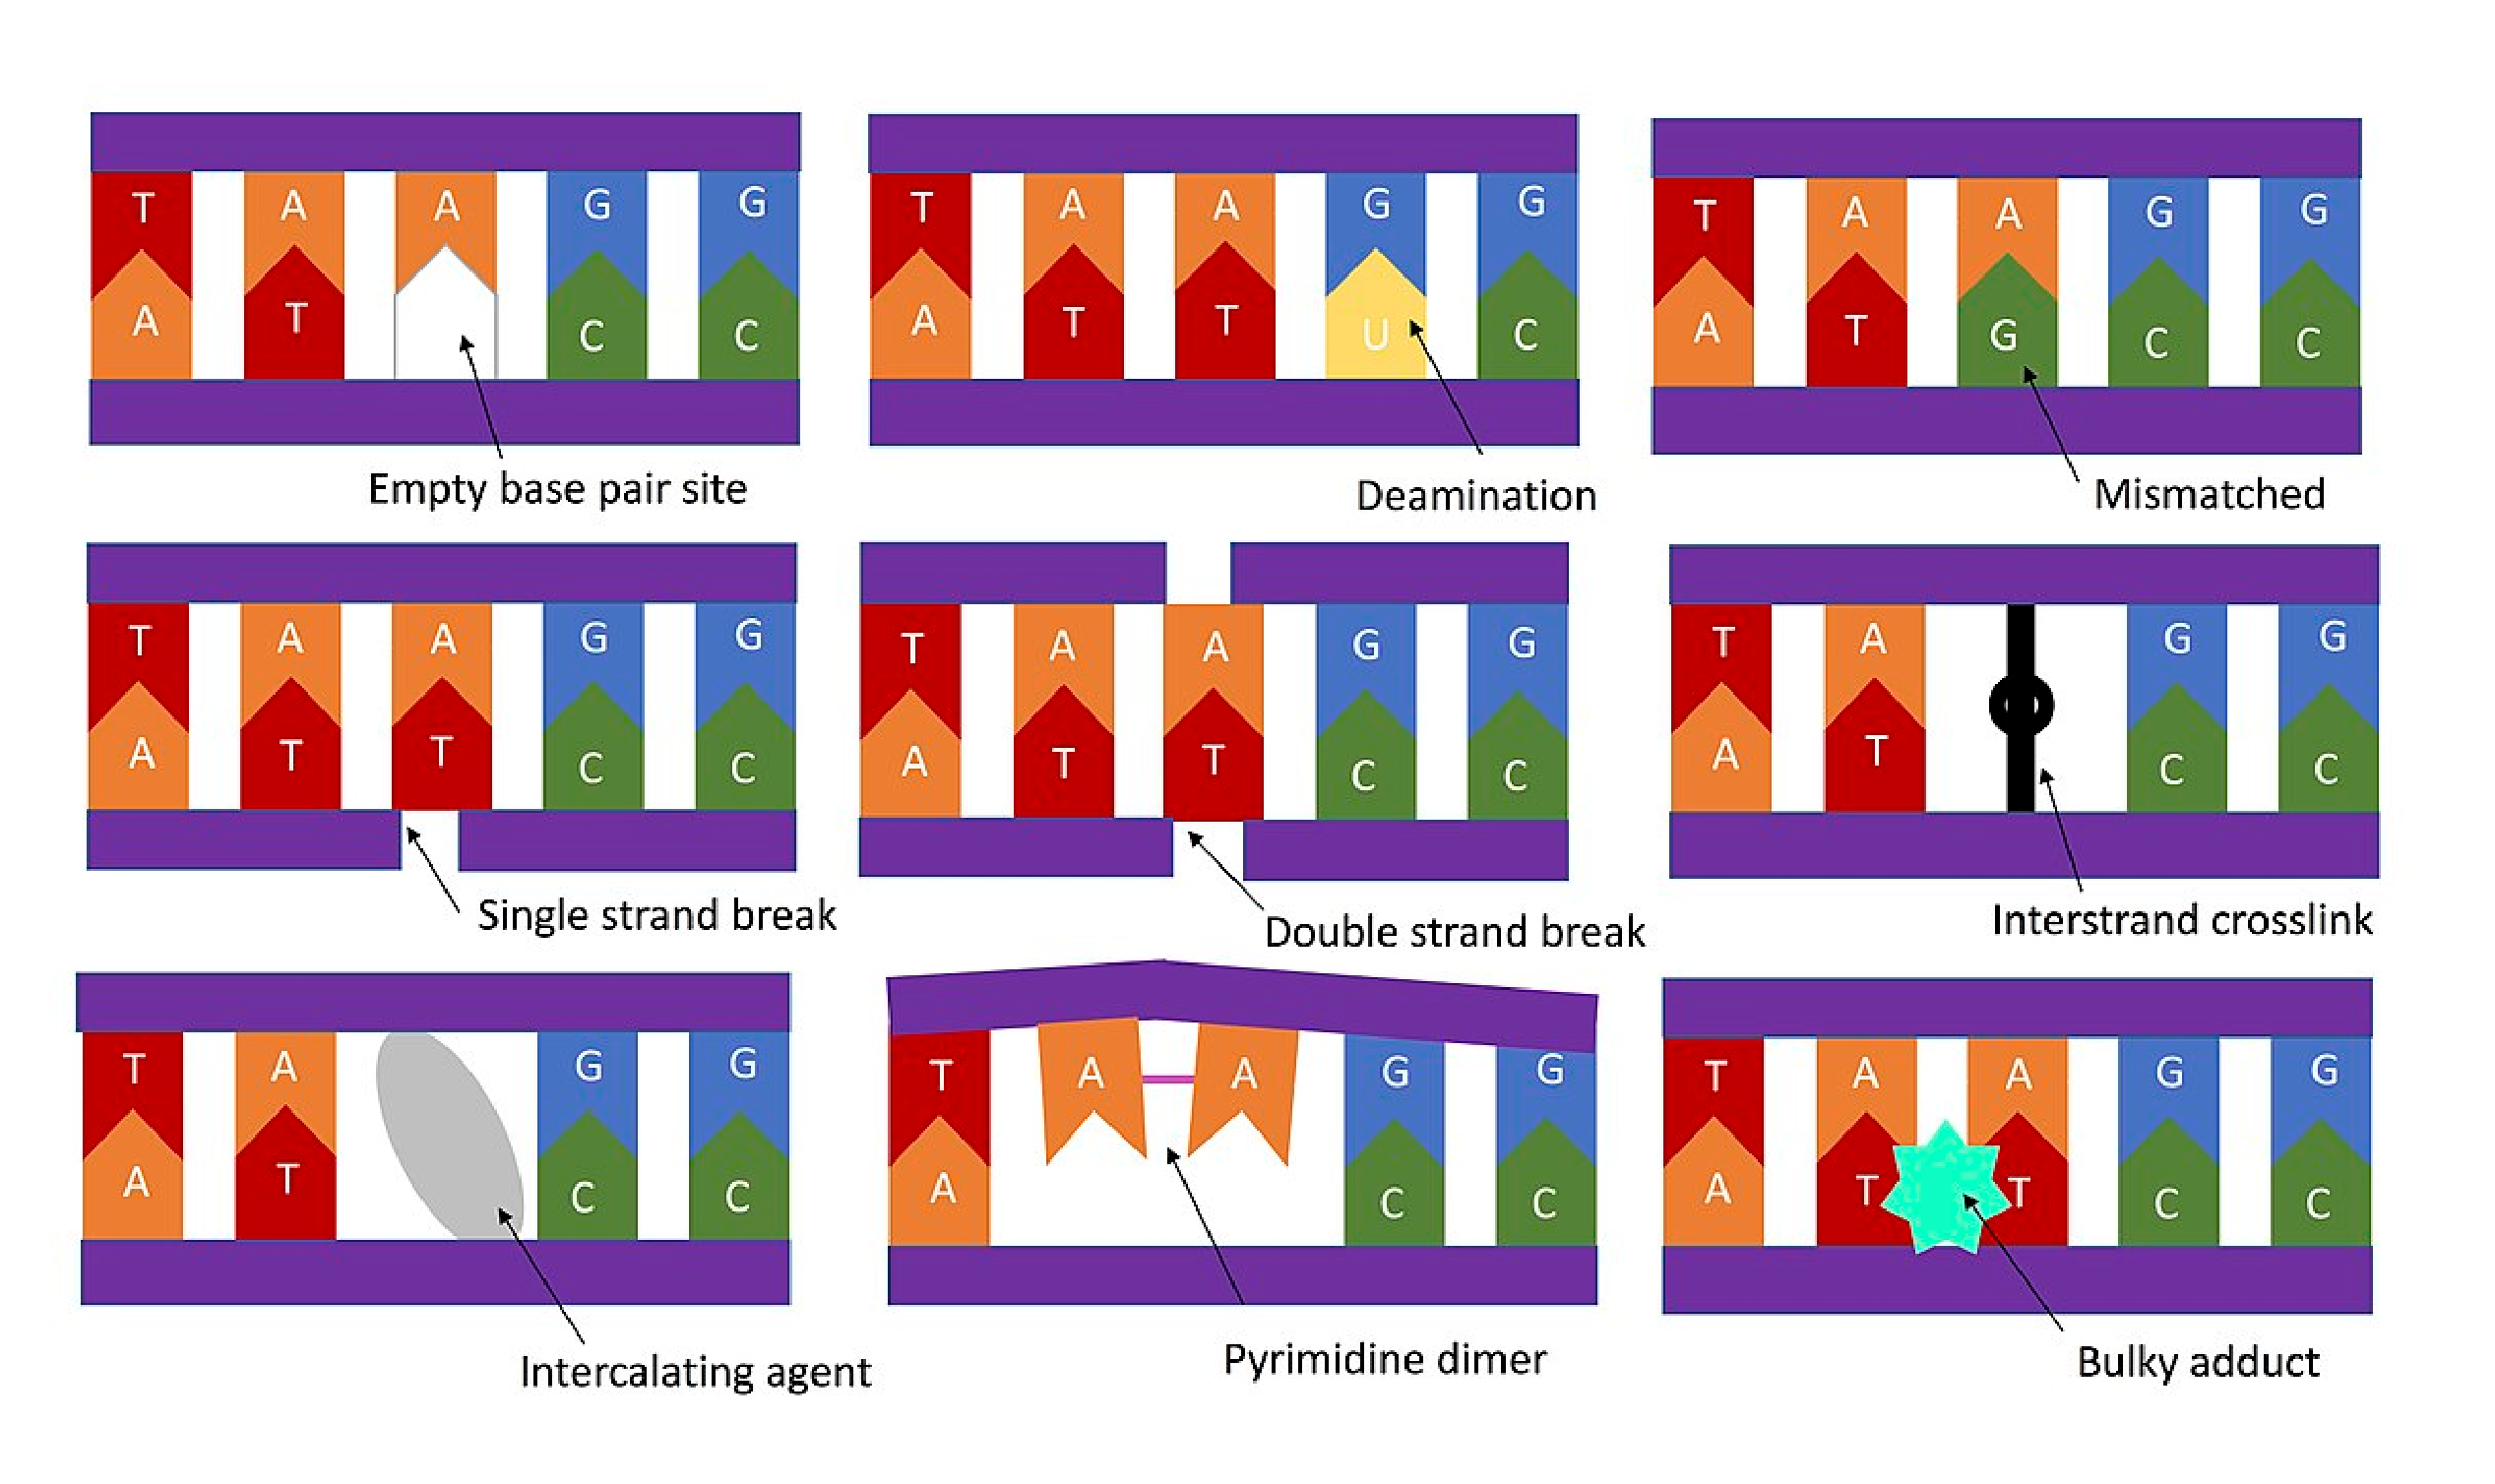
\includegraphics[width=1.0\textwidth]{mmr/Types_of_DNA_Damage}
%  \caption[Various types of DNA damage.]{Various types of DNA damage. The upper row shows a DNA mismatch (the example used here) in the upper row on the right. In the upper row centre incorporation of a Uracil base is shown, which was modelled in \cite{10.1007/978-3-319-99498-7_8}.  \href{https://commons.wikimedia.org/wiki/File:Types_of_DNA_Damage.jpg}{Image} by Chantelmao is licensed under \href{https://creativecommons.org/licenses/by-sa/4.0/deed.en}{CC-BY-SA-4.0}.}
%  \label{fig:damages}
%\end{figure}

Coming back to the DNA mismatch repair mentioned in the introduction, we first give a detailled explanation of how it happens. Such a repair is not possible in the same way as the base excision repair (BER), since any of the two bases could be wrong, so the non-matching  bases do not tell what to do. In contrast, to repair the incorporation of a uracil, clearly the uracil must be removed and replaced. A description of the process on an abstract level is as follows: If two bases are incorporated into a DNA strand which do not match (i.e. are not C/G or A/T pairs), this constitutes a defect in the DNA strand. A repair similar to BER is not possible, since it is not clear which of the two bases is correct just from the bases alone - both could be right. We are looking at a specific way to handle this situation, called Methyl Mismatch Repair (MMR). This is the repair mechanism in bacteria, in particular E. coli, for which detailed studies has been done.\footnote{Paul L. Modrich, Tomas Lindahl and Aziz Sancar received the Nobel Price in Chemistry 2015 for their work on DNA repair. Modrich's Nobel Lecture about Methyl-directed Mismatch Repair in E. coli and humans \cite{pmid27198632} gives a nice overview.} This process is based on DNA strands being methylated sometime after their creation. Methylation means the attachment a methyl group (a carbon atom with three hydrogen atoms), in this case to the adenine base. Specifically, this happens whenever there is a GATC sequence. Since the methylation (which is done by specific proteins, which we do not model) happens with a delay after the duplication of a strand, for some time the old strand is methylated, the new strand is not. This enables the removal of exactly the new base, which must be the wrong one.

The actual repair involves the proteins MutS, MutL, MutH, and UvrD. MutS first binds to the mismatch and then recruits MutL and MutH. MutL can detected the methylated strand and can form a loop in the DNA. In this loop, the newer strand now is outside, whereas the old strand is covered by itself and MutL. MutH cleaves the unmethylated strand. This happens in some distance from the mismatch, due to the size of the proteins and the loop in the DNA. UvrD can then detect the cleavage and can move along the strand. It removes the outer strand when moving along. At the same time, the MutL, MutH, and MutS proteins are released and the loop in the DNA disappears. UvrD moves to after the mismatch, removing the wrong base together with their neighbours. UvrD then goes off the DNA and leaves the old, and correct, strand to be completed. 

\subsection{Modelling DNA Mismatch Repair}

For modelling MMR, we use the components from \cite{10.1007/978-3-319-99498-7_8} as much as possible. We reuse the deoxyribose/phosphate groups, and the four bases A, T, C, and G. We will extend those components where needed, but we will keep the original actions. Overall, in order to model MMR, we need the following components: deoxyribose/phosphate groups, the four bases A, T, G, C, the methyl group Me, and the proteins MutS, MutL, MutH, and UvrD. The reused components are the following:
%
$$\begin{array}{lll}
DP & \bydef & )(p3,p5;s) \paral (b,d)).DP'\\
A & \bydef & (b;i).(a,m;r).A'\\
T & \bydef & (b;i).(t;r).T'\\
G & \bydef & (b;i).(g;r).G'\\
C & \bydef & (b;i).(c;r).C'\\
\end{array}$$
%
where processes $A$, $T$, $G$, and $C$ model the bases adenine (A), cytosine (C), guanine (G), and thymine (T). Notice we have added actions $s$, $m$, and $r$. $m$ is enabling the methylation. It only exists in $A$, since the methylation is only happending there. Also, the actions on DP have been regrouped (but all original actions are still there). In $DP$, we are now using a parallel operator. This is necessary to enable a breaking of a bond to $p3$ or $p5$ whilst there is still a bond to $b$. The action $d$, which was used by UDG in the modelling of BER is not used here, as we will see. We keep it to have an extension of the previous modelling.

We also need additional components, namely the methyl group, the MutS, MutL, MutH, and UvrD proteins. We model these as follows:
$$\begin{array}{lll}
Me & \bydef & (m).(n).Me'\\
MutS & \bydef & (k,k).(l).MutS'\\
MutL & \bydef & (l).(n).(o).MutL'\\
MutH & \bydef & (o).(w).MutH'\\
UvrD & \bydef & ((u;r) \paral (v;s)).UvrD'\\
\end{array}$$
%
where processes $MutS$, $MutL$, $MutH$, and $UvrD$ model the MutS, MutL, MutH, and UvrD protein respectively.  Here $s$, $i$, and $r$ are weak actions, all other actions, namely $p3$, $p5$, $b$, $d$, $a$, $t$, $g$, $c$, $m$, $n$, $k$, $l$, $o$, $s$, $u$, $v$ and $w$, are strong. Notice that $i$ is not used, but we keep it to have this model as an extension of the BER model. In $UvrD$, we again use a  parallel operator. This will make it possible for UvrD to break two bonds with every ``step'' it moves.


The synchronisation function for our system is as follows:
%
\[\arraycolsep=3.4pt\def\arraystretch{1.0}
\begin{array}{ l c l | l c l | l c l | l c l}
\gamma(p3,p5) & = & p & \gamma(b,b) & = & bb & \gamma(a,t) & = & at &  \gamma(g,c) & = & gc \\
\hline
\gamma(m,m) & = & mm & \gamma(k,a) & = & ka & \gamma(k, g) & = & kg & \gamma(k,c) & = & kc \\
\hline
\gamma(k,t) & = & kt & \gamma(l,l) & = & ll &\gamma(n,n) & = & nn & \gamma(o,o) & = & oo\\
\hline
\gamma(r,r) & = & rr & \gamma(t,u) & = & tu &\gamma(p,s) & = & ps &\gamma(w,s) & = & ws\\
\hline
\gamma(v,p3) & = & vp3 &  \gamma(u,r) & = & ur  & \gamma(s,v) & = & sv & & & \\
\end{array}
\]

As before, the deoxyribose/phosphate groups and the bases can combine to form a DNA strand. In that strand, there can be DNA mismatches. Note that we do not model how they happen, we just assume a DNA strand as in Figure~\ref{fig:state1} with a DNA mismatch and correct pairs otherwise. The mismatch here is an A-G pair, but that is not crucial for our modelling. The A-G bases cannot bond to each other, that is the case in our modelling as well in reality, and this gives the opportunity for the repair. To the left of the DNA strand, there is a CTAG sequence (respectively a GATC sequence). This is where the methylation happens. In our case, we have a recently duplicated strand, where the older part is the upper one (A is methylated) and the newer part is the lower one (A is not methylated). The methylation itself is done by proteins which are not modelled here. This is the situation where the MMR can happen.

\begin{figure}[h!]
\psfrag{dp1}{$DP_1$}
\psfrag{dp2}{$DP_2$}
\psfrag{dp3}{$DP_3$}
\psfrag{dp4}{$DP_4$}
\psfrag{dp5}{$DP_5$}
\psfrag{dp6}{$DP_6$}
\psfrag{dp7}{$DP_7$}
\psfrag{dp8}{$DP_8$}
\psfrag{dp9}{$DP_9$}
\psfrag{dp10}{$DP_{10}$}
\psfrag{dp11}{$DP_{11}$}
\psfrag{dp12}{$DP_{12}$}
%\psfrag{A1}[cc][][0.8][0]{{$\mathit{A_1}}$}
\psfrag{A1}[cc][][0.8][0]{$A_1$}
\psfrag{A2}[cc][][0.8][0]{$A_2$}
\psfrag{A3}[cc][][0.8][0]{$A_3$}
\psfrag{T1}[cc][][0.8][0]{$T_1$}
\psfrag{T2}[cc][][0.8][0]{$T_2$}
\psfrag{C1}[cc][][0.8][0]{$C_1$}
\psfrag{C2}[cc][][0.8][0]{$C_2$}
\psfrag{C3}[cc][][0.8][0]{$C_3$}
\psfrag{G1}[cc][][0.8][0]{$G_1$}
\psfrag{G2}[cc][][0.8][0]{$G_2$}
\psfrag{G3}[cc][][0.8][0]{$G_3$}
\psfrag{G4}[cc][][0.8][0]{$G_4$}
\psfrag{Me}{${\mathit{Me}}$}
\psfrag{MS}{${\mathit{MutS}}$}
\psfrag{ML}{${\mathit{MutL}}$}
\psfrag{MH}{${\mathit{MutH}}$}
\psfrag{UD}{${\mathit{UvrD}}$}
  \centering
    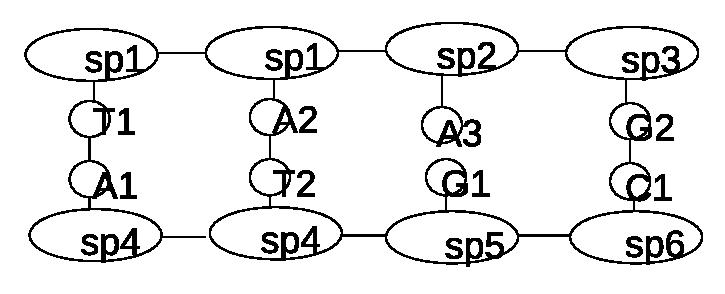
\includegraphics[width=1.0\textwidth]{mmr/state1}
  \caption[A six base pair DNA fragment.]{A six base pair DNA fragment, with a DNA mismatch and methylation of one strand. The proteins MutL, MutS, MutH, and UvrD are currently not bound to the DNA.}
  \label{fig:state1}
\end{figure}

We can model this similar to what we did before as:

$$\begin{array}{l}
(DP_1 \paral DP_2 \paral DP_3 \paral DP_4 \paral DP_5 \paral DP_6 \paral \\
C_1 \paral T_1 \paral A_1 \paral G_1 \paral A_2 \paral C_2 \paral \\
G_2 \paral A_3 \paral T_2 \paral C_3 \paral G_3 \paral G_4 \paral \\
DP_7 \paral DP_8 \paral DP_9 \paral DP_{10} \paral DP_{11} \paral DP_{12} \paral \\
Me \paral MutS \paral MutL \paral MutH \paral UvrD) \\
\setminus\{p3, p5, s, i, r, b, b, d, b, a, t, g, c, m, n, k, l, o, s, u, v, w\} 
\end{array}$$ 

We leave out the restriction from now on for ease of reading. We number actions using subscripts where there is more than one instance, and set initial bonds as required. We get the following process:
%
\begin{flalign*}
&((p3_1,p5_1[1];s_1) \paral (b_1[10],d_1)).DP_1' \paral ((p3_2[1],p5_2[2];s_2) \paral (b_2[8],d_2)).DP_2' \paral &&\\
&((p3_3[2],p5_3[3];s_3) \paral (b_3[6],d_3)).DP_3' \paral ((p3_4[3],p5_4[4];s_4) \paral (b_4[9],d_4)).DP_4' \paral &&\\
&((p3_5[4],p5_5[5];s_5) \paral (b_5[7],d_5)).DP_5' \paral ((p3_6[5],p5_6;s_6) \paral (b_6[11],d_6)).DP_6' \paral  &&\\
&(b_{10}[10];i_{10}).(c_1[41];r_{10}).C_1' \paral (b_4[8];i_4).(t_1[23]:r_4).T_1' \paral (b_1[6];i_1).(a_1[24],m_1[40];r_1).A_1' \paral &&\\
& (b_6[9];i_6).(g_1[25];r_6).G_1' \paral (b_2[7];i_2).(a_2,m_2;r_2).A_2' \paral (b_{11}[11];i_{11}).(c_2[27];r_{11}).C_2' \paral &&\\
&(b_7[17];i_7).(g_2[41];r_7).G_2' \paral (b_3[18];i_3).(a_3[23],m_3;r_3).A_3' \paral (b_5[19];i_5).(t_2[24];r_5).T_2' \paral   &&\\
& (b_{12}[20];i_{12}).(c_3[25];r_{12}).C_3'  \paral (b_8[21];i_8).(g_3;r_8).G_3' \paral (b_9[22];i_9).(g_4[27];r_9).G_4' \paral&&\\
&((p3_7,p5_7[12];s_7) \paral (b_7[17],d_7)).DP_7' \paral ((p3_8[12],p5_8[13];s_8) \paral (b_8[18],d_8)).DP_8' \paral &&\\
&((p3_9[13],p5_9[14];s_9) \paral (b_9[19],d_9)).DP_9' \paral ((p3_{10}[14],p5_{10}[15];s_{10}) \paral (b_{10}[20],d_{10})).DP_{10}' \paral  &&\\
&((p3_{11}[15],p5_{11}[16];s_{11}) \paral (b_{11}[21],d_{11})).DP_{11}' \paral ((p3_{12}[16],p5_{12};s_{12}) \paral (b_{12}[22],d_{12})).DP_{12}' \paral  &&\\
&(m[40]).(n).Me'\paral (k,k).(l).MutS' \paral (l).(n).(o).MutL' \paral &&\\
&(o).(w).MutH' \paral (u;r) \paral (v;s).UvrD'&&
\end{flalign*}

In this short DNA section , we firstly have a mismatch - $A_2$ and $G_3$ do not form an A/T or G/C pair as required. Secondly, methylation has happened on the old half of the strand, which means that an methyl group ($Me$) is attached to $A_1$. Note that there is no methyl group on $A_2$. This is because the methylation only happens on CTAG sequences. This happens via a specific protein, which we do not model, we just assume the end result. No $A$s would be methylated on the new half, even if they were in a CTAG sequence, since not enough time has passed for this to happen.

Since $DP_1$, $DP_2$, $DP_3$, $DP_4$, $DP_5$, $DP_6$, $DP_7$, $C_1$,  $T_1$, $C_2$, $G_2$, $A_3$, and $G_4$ never directly participate in a transition, we will not write these in the future in order to keep the notation compact. They still are part of the system, and can be added without any changes to the rest. 

MutS can now bond to the $A$ and $G$ bases,  specifically to processes $A_2$ and $G_3$  via the $a_2$ and $g_3$ actions. This is the recognition of the mismatch. Note that the $a$ and $g$ actions are not available on matching pairs. So the bonding is not possible if the bases are properly paired, and also not if a Uracil is incorporated into the strand (as in the BER example). The transitions for creating the two bonds between $MutS$ and
$A_2$ and $G_3$ are as follows:

\begin{flalign*}
&\xrightarrow{ka[28]} \xrightarrow{kg[29]} (b_1[6];i_1).(a_1[24],m_1[40];r_1).A_1' \paral (b_6[9];i_6).(g_1[25];r_6).G_1' \paral &&\\
&(b_2[7];i_2).(\mathbf{a_2[28]},m_2;r_2).A_2' \paral  (b_5[19];i_5).(t_2[24];r_5).T_2' \paral (b_{12}[20];i_{12}).(c_3[25];r_{12}).C_3'  \paral &&\\
&(b_8[21];i_8).(\mathbf{g_3[29]};r_8).G_3' \paral ((p3_8[12],p5_8[13];s_8) \paral (b_8[18],d_8)).DP_8' \paral &&\\
&((p3_9[13],p5_9[14];s_9) \paral (b_9[19],d_9)).DP_9' \paral ((p3_{10}[14],p5_{10}[15];s_{10}) \paral (b_{10}[20],d_{10})).DP_{10}' \paral &&\\
&((p3_{11}[15],p5_{11}[16];s_{11}) \paral (b_{11}[21],d_{11})).DP_{11}' \paral ((p3_{12}[16],p5_{12};s_{12}) \paral (b_{12}[22],d_{12})).DP_{12}' \paral  &&\\
&(m[40]).(n).Me'\paral (\mathbf{k[28],k[29]}).(l).MutS' \paral (l).(n).(o).MutL' \paral &&\\
&(o).(w).MutH' \paral ((u;r) \paral (v;s)).UvrD'&&
\end{flalign*}

Now it is possible for $MutL$ to bond to $MutS$ via a synchronisation on $l$ with key 30:

\begin{flalign*}
&\xrightarrow{ll[30]} (b_1[6];i_1).(a_1[24],m_1[40];r_1).A_1' \paral (b_6[9];i_6).(g_1[25];r_6).G_1' \paral &&\\
&(b_2[7];i_2).(a_2[28],m_2;r_2).A_2' \paral (b_5[19];i_5).(t_2[24];r_5).T_2' \paral  (b_{12}[20];i_{12}).(c_3[25];r_{12}).C_3'  \paral &&\\
&(b_8[21];i_8).(g_3[29];r_8).G_3' \paral ((p3_8[12],p5_8[13];s_8) \paral (b_8[18],d_8)).DP_8' \paral &&\\
&((p3_9[13],p5_9[14];s_9) \paral (b_9[19],d_9)).DP_9' \paral ((p3_{10}[14],p5_{10}[15];s_{10}) \paral (b_{10}[20],d_{10})).DP_{10}' \paral  &&\\
&((p3_{11}[15],p5_{11}[16];s_{11}) \paral (b_{11}[21],d_{11})).DP_{11}' \paral ((p3_{12}[16],p5_{12};s_{12}) \paral (b_{12}[22],d_{12})).DP_{12}' \paral &&\\
&(m[40]).(n).Me'\paral (k[28],k[29]).(\mathbf{l[30]}).MutS' \paral (\mathbf{l[30]}).(n).(o).MutL' \paral &&\\
&(o).(w).MutH' \paral ((u;r) \paral (v;s)).UvrD'&&
\end{flalign*}

$MutL$ now can bond with $Me$ via $n$, which means it detects which of the strands is methylated, and therefore the correct one:

\begin{flalign*}
&\xrightarrow{nn[31]} (b_1[6];i_1).(a_1[24],m_1[40];r_1).A_1' \paral (b_6[9];i_6).(g_1[25];r_6).G_1' \paral &&\\
&(b_2[7];i_2).(a_2[28],m_2;r_2).A_2' \paral (b_5[19];i_5).(t_2[24];r_5).T_2' \paral  (b_{11}[20];i_{11}).(c_3[25];r_{12}).C_3'  \paral&&\\
&(b_8[21];i_8).(g_2[29];r_8).G_3' \paral ((p3_8[12],p5_8[13];s_8) \paral (b_8[18],d_8)).DP_8' \paral &&\\
&((p3_9[13],p5_9[14];s_9) \paral (b_9[19],d_9)).DP_9' \paral ((p3_{10}[14],p5_{10}[15];s_{10}) \paral (b_{10}[20],d_{10})).DP_{10}' \paral &&\\
&((p3_{11}[15],p5_{11}[16];s_{11}) \paral (b_{11}[21],d_{11})).DP_{11}' \paral ((p3_{12}[16],p5_{12};s_{12}) \paral (b_{12}[22],d_{12})).DP_{12}' \paral  &&\\
&S(m[40]).(\mathbf{n[31]}).Me'\paral (k[28],k[29]).(l[30]).MutS' \paral (l[30]).(\mathbf{n[31]}).(o).MutL' \paral &&\\
&(o).(w).MutH' \paral ((u;r) \paral (v;s)).UvrD'&&
\end{flalign*}

MutL is now ready to recruit MutH:

\begin{flalign*}
&\xrightarrow{oo[32]} (b_1[6];i_1).(a_1[24],m_1[40];r_1).A_1' \paral (b_6[9];i_6).(g_1[25];r_6).G_1' \paral  &&\\
&(b_2[7];i_2).(a_2[28],m_2;r_2).A_2' \paral (b_5[19];i_5).(t_2[24];r_5).T_2' \paral (b_{12}[20];i_{12}).(c_3[25];r_{12}).C_3'  \paral&&\\
&(b_8[21];i_8).(g_3[29];r_8).G_3' \paral ((p3_8[12],p5_8[13];s_8) \paral (b_8[18],d_8)).DP_8' \paral &&\\
&((p3_9[13],p5_9[14];s_9) \paral (b_9[19],d_9)).DP_9' \paral ((p3_{10}[14],p5_{10}[15];s_{10}) \paral (b_{10}[20],d_{10})).DP_{10}' \paral &&\\
& ((p3_{11}[15],p5_{11}[16];s_{11}) \paral (b_{11}[21],d_{11})).DP_{11}' \paral ((p3_{12}[16],p5_{12};s_{12}) \paral (b_{12}[22],d_{12})).DP_{12}' \paral &&\\
&(m[40]).(n[31]).Me'\paral (k[28],k[29]).(l[30]).MutS' \paral (l[30]).(n[31]).(\mathbf{o[32]}).MutL' \paral &&\\
&(\mathbf{o[32]}).(w).MutH' \paral ((u;r) \paral (v;s)).UvrD'&&
\end{flalign*}

MutH is now ready to cleave the DNA at the right location:

\begin{flalign*}
&\xrightarrow{\{ws[33],\underline{p}[13]\}} (b_1[6];i_1).(a_1[24],m_1[40];r_1).A_1' \paral (b_6[9];i_6).(g_1[25];r_6).G_1' \paral  &&\\
&(b_2[7];i_2).(a_2[28],m_2;r_2).A_2' \paral (b_5[19];i_5).(t_2[24];r_5).T_2' \paral (b_{12}[20];i_{12}).(c_3[25];r_{12}).C_3'  \paral&&\\
&(b_8[21];i_8).(g_3[29];r_8).G_3' \paral ((p3_8[12],\mathbf{p5_8};s_8) \paral (b_8[18],d_8)).DP_8' \paral &&\\
&((\mathbf{p3_9},p5_9[14];\mathbf{s_9[33]}) \paral (b_9[19],d_9)).DP_9' \paral ((p3_{10}[14],p5_{10}[15];s_{10}) \paral (b_{10}[20],d_{10})).DP_{10}' \paral  &&\\
&((p3_{11}[15],p5_{11}[16];s_{11}) \paral (b_{11}[21],d_{11})).DP_{11}' \paral ((p3_{12}[16],p5_{12};s_{12}) \paral (b_{12}[22],d_{12})).DP_{12}' \paral  &&\\
&(m[40]).(n[31]).Me'\paral (k[28],k[29]).(l[30]).MutS' \paral (l[30]).(n[31]).(o[32]).MutL' \paral &&\\
&(o[32]).(\mathbf{w[33]}).MutH' \paral ((u;r) \paral (v;s)).UvrD'&&
\end{flalign*}

Next, {\em promotion} happens, which moves the bond with key 33 from weak action $s_9$ to strong action $p3_9$:

\begin{flalign*}
&\overset{ \rulename{prom}}\Rightarrow (b_1[6];i_1).(a_1[24],m_1[40];r_1).A_1' \paral (b_6[9];i_6).(g_1[25];r_6).G_1' \paral  &&\\
&(b_2[7];i_2).(a_2[28],m_2;r_2).A_2' \paral (b_5[19];i_5).(t_2[24];r_5).T_2' \paral (b_{12}[20];i_{12}).(c_3[25];r_{10}).C_3'  \paral &&\\
&(b_8[21];i_8).(g_3[29];r_8).G_3' \paral ((p3_8[12],p5_8;s_8) \paral (b_8[18],d_8)).DP_8' \paral &&\\
&((\mathbf{p3_9[33]},p5_9[14];\mathbf{s_9}) \paral (b_9[19],d_9)).DP_9' \paral ((p3_{10}[14],p5_{10}[15];s_{10}) \paral (b_{10}[20],d_{10})).DP_{10}' \paral  &&\\
&((p3_{11}[15],p5_{11}[16];s_{11}) \paral (b_{11}[21],d_{11})).DP_{11}' \paral ((p3_{12}[16],p5_{12};s_{12}) \paral (b_{12}[22],d_{12})).DP_{12}' \paral  &&\\
&(m[40]).(n[31]).Me'\paral (k[28],k[29]).(l[30]).MutS' \paral (l[30]).(n[31]).(o[32]).MutL' \paral &&\\
&(o[32]).(\mathbf{w[33]}).MutH' \paral ((u;r) \paral (v;s)).UvrD'&&
\end{flalign*}

Note that execution of $s_9$ on $DP_9$ leads to breaking a bond between two deoxyribose/phosphate groups. Specifically, bond 33 from $MutH$ to $DP_9$ via actions $w$ and $s$ is formed and bond 13 between $p5$ in $DP_8$ and $p3$ in  $DP_9$ is broken. We use a concerted action and rewriting for this. The situation after this step is shown in Figure~\ref{fig:state2}. This has now the right DNA strand cleaved.

\begin{figure}[h!]
\psfrag{dp1}{$DP_1$}
\psfrag{dp2}{$DP_2$}
\psfrag{dp3}{$DP_3$}
\psfrag{dp4}{$DP_4$}
\psfrag{dp5}{$DP_5$}
\psfrag{dp6}{$DP_6$}
\psfrag{dp7}{$DP_7$}
\psfrag{dp8}{$DP_8$}
\psfrag{dp9}{$DP_9$}
\psfrag{dp10}{$DP_{10}$}
\psfrag{dp11}{$DP_{11}$}
\psfrag{dp12}{$DP_{12}$}
\psfrag{A1}[cc][][0.8][0]{$A_1$}
\psfrag{A2}[cc][][0.8][0]{$A_2$}
\psfrag{A3}[cc][][0.8][0]{$A_3$}
\psfrag{T1}[cc][][0.8][0]{$T_1$}
\psfrag{T2}[cc][][0.8][0]{$T_2$}
\psfrag{C1}[cc][][0.8][0]{$C_1$}
\psfrag{C2}[cc][][0.8][0]{$C_2$}
\psfrag{C3}[cc][][0.8][0]{$C_3$}
\psfrag{G1}[cc][][0.8][0]{$G_1$}
\psfrag{G2}[cc][][0.8][0]{$G_2$}
\psfrag{G3}[cc][][0.8][0]{$G_3$}
\psfrag{G4}[cc][][0.8][0]{$G_4$}
\psfrag{Me}{${\mathit{Me}}$}
\psfrag{MS}{${\mathit{MutS}}$}
\psfrag{ML}{${\mathit{MutL}}$}
\psfrag{MH}{${\mathit{MutH}}$}
\psfrag{UD}{${\mathit{UvrD}}$}
  \centering
    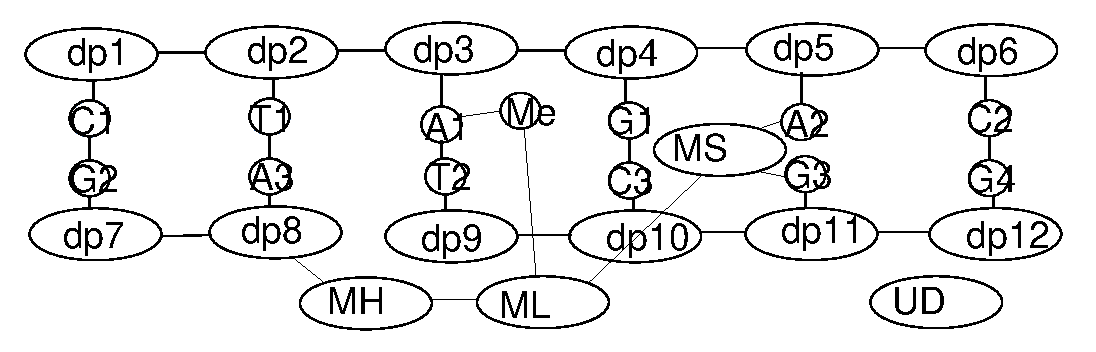
\includegraphics[width=1.0\textwidth]{mmr/state2}
  \caption[A six base pair DNA fragment.]{A six base pair DNA fragment, with a DNA mismatch and methylation of one strand. The mismatch has been detected by MutS and MutH and MutL have been recruited. MutL has detected the methylation, and MutH has cleaved the strand containing the wrong base.}
  \label{fig:state2}
\end{figure}

Now the UvrD protein can use the cleavage to remove pairs of deoxyribose/phosphate groups and bases. This works as follows:

\begin{flalign*}
&\xrightarrow{\{sv[34],\underline{at}[14]\}}  \overset{ \rulename{prom}}\Rightarrow \xrightarrow{\{ur[35],\underline{at}[24]\}}  \overset{ \rulename{prom}}\Rightarrow (b_1[6];i_1).(\mathbf{a_1},m_1[40];r_1).A_1' \paral  (b_6[9];i_6).(g_1[25];r_6).G_1' \paral &&\\
&(b_2[7];i_2).(a_2[28],m_2;r_2).A_2' \paral (b_5[19];i_5).(\mathbf{t_2[35]};r_5).T_2' \paral (b_{12}[20];i_{12}).(c_3[25];r_{12}).C_3'  \paral&&\\
&(b_8[21];i_8).(g_3[29];r_8).G_3' \paral ((p3_8[12],p5_8;s_8) \paral (b_8[18],d_8)).DP_8' \paral &&\\
&((p3_9[33],p5_9;s_9) \paral (b_9[19],d_9)).DP_9' \paral ((\mathbf{p3_{10}[34]},p5_{10}[15];s_{10}) \paral (b_{10}[20],d_{10})).DP_{10}' \paral  &&\\
&((p3_{11}[15],p5_{11}[16];s_{11}) \paral (b_{11}[21],d_{11})).DP_{11}' \paral ((p3_{12}[16],p5_{12};s_{12}) \paral (b_{12}[22],d_{12})).DP_{12}' \paral  &&\\
&(m[40]).(n[31]).Me'\paral (k[28],k[29]).(l[30]).MutS' \paral (l[30]).(n[31]).(o[32]).MutL' \paral &&\\
&(o[32]).(w[33]).MutH' \paral ((\mathbf{u[35]};r) \paral (\mathbf{v[34]};s)).UvrD'&&
\end{flalign*}

$UD$ is attached not to $DP_9$ initially here, but to $DP_10$. If it would be attached to $DP_9$, it would have no connection to the DNA strand anymore once the bonds of $DP_9$ and $T_2$ to the DNA strand are broken.

The removal of the first base and deoxyribose/phosphate group is shown in Figure~\ref{fig:state3}. The dashed lines indicate the bonds being broken and formed during concerted actions. The two concerted actions are shown by thin (34/14) and bold dashed lines (35/24).

\begin{figure}[h!]
\psfrag{dp1}{${DP_1}$}
\psfrag{dp2}{${DP_2}$}
\psfrag{dp3}{${DP_3}$}
\psfrag{dp4}{${DP_4}$}
\psfrag{dp5}{${DP_5}$}
\psfrag{dp6}{${DP_6}$}
\psfrag{dp7}{${DP_7}$}
\psfrag{dp8}{${DP_8}$}
\psfrag{dp9}{${DP_9}$}
\psfrag{dp10}{${DP_{10}}$}
\psfrag{dp11}{${DP_{11}}$}
\psfrag{dp12}{${DP_{12}}$}
\psfrag{A1}[cc][][0.8][0]{${A_1}$}
\psfrag{A2}[cc][][0.8][0]{${A_2}$}
\psfrag{A3}[cc][][0.8][0]{${A_3}$}
\psfrag{T1}[cc][][0.8][0]{${T_1}$}
\psfrag{T2}[cc][][0.8][0]{${T_2}$}
\psfrag{C1}[cc][][0.8][0]{${C_1}$}
\psfrag{C2}[cc][][0.8][0]{${C_2}$}
\psfrag{C3}[cc][][0.8][0]{${C_3}$}
\psfrag{G1}[cc][][0.8][0]{${G_1}$}
\psfrag{G2}[cc][][0.8][0]{${G_2}$}
\psfrag{G3}[cc][][0.8][0]{${G_3}$}
\psfrag{G4}[cc][][0.8][0]{${G_4}$}
\psfrag{Me}{${\mathit{Me}}$}
\psfrag{MS}{${\mathit{MutS}}$}
\psfrag{ML}{${\mathit{MutL}}$}
\psfrag{MH}{${\mathit{MutH}}$}
\psfrag{UD}{${\mathit{UvrD}}$}
  \centering
    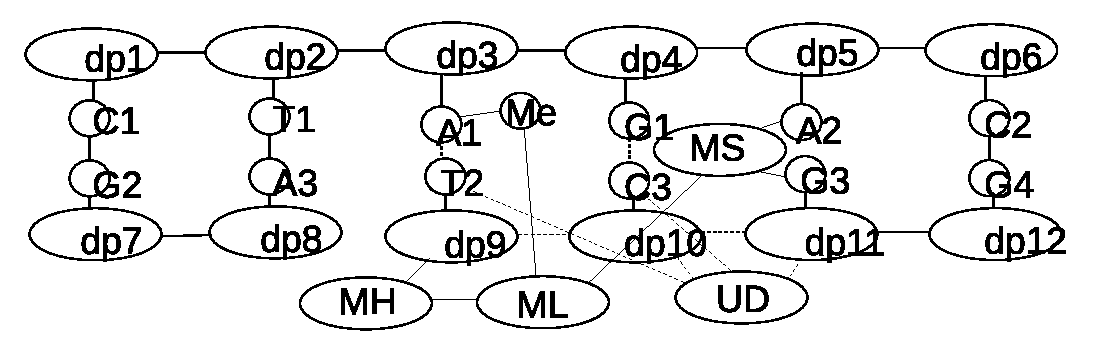
\includegraphics[width=1.0\textwidth]{mmr/state3}
  \caption[A six base pair DNA fragment.]{A six base pair DNA fragment, with a DNA mismatch and methylation of one strand. UvrD has now bonded to $T_2$ and $DP_{10}$, breaking the bonds of those molecules to the rest of the DNA via concerted actions (shown as dotted lines). In a next step, UvrD can now ``walk'' along the DNA strand, and remove the next pair.}
  \label{fig:state3}
\end{figure}

From here, UvrD can ``walk'' along the strand. As opposed to BER, the bonds between the base pairs are now broken during the walk. In parallel, the bonds between the deoxyribose/phosphate groups are also broken as UvrD progresses. We write this as two separate concerted transitions here for clarity:

\begin{flalign*}
&\xrightarrow{\{ss[36],\underline{vp3}[34],\underline{p}[15]\}} \overset{ \rulename{prom}}\Rightarrow  (b_1[6];i_1).(a_1,m_1[40];r).A_1' \paral (b_6[9];i_6).(g_1[25];r_3).G_1' \paral &&\\
&(b_2[7];i_2).(a_2[28],m_2;r).A_2' \paral (b_5[19];i_5).(t_2[35];r_2).T_2' \paral (b_{11}[20];i_{11}).(c_3[25];r_8).C_3'  \paral&&\\
&(b_8[21];i_8).(g_2[29];r_4).G_3' \paral ((p3_8[12],p5_8;s_8) \paral (b_8[18],d_8)).DP_8' \paral &&\\
&((p3_9[33],p5_9;s_9) \paral (b_9[19],d_9)).DP_9' \paral ((\mathbf{p3_{10},p5_{10}};s_{10}) \paral (b_{10}[20],d_{10})).DP_{10}' \paral &&\\
&((\mathbf{p3_{11}[36]},p5_{11}[16];s_{11}) \paral (b_{11}[21],d_{11})).DP_{11}' \paral ((p3_{12}[16],p5_{12};s_{12}) \paral (b_{12}[22],d_{12})).DP_{12}' \paral  &&\\
&(m[40]).(n[31]).Me'\paral (k[28],k[29]).(l[30]).MutS' \paral (l[30]).(n[31]).(o[32]).MutL' \paral &&\\
&(o[32]).(w[33]).MutH' \paral ((u[35];r) \paral (\mathbf{v[36]};s)).UvrD'&&
\end{flalign*}

\begin{flalign*}
&\xrightarrow{\{rr[37],\underline{tu}[35],\underline{cg}[25]\}} \overset{ \rulename{prom}}\Rightarrow  (b_1[6];i_1).(a_1,m_1[40];r).A_1' \paral (b_6[9];i_6).(\mathbf{g_1};r_3).G_1' \paral  &&\\
&(b_2[7];i_2).(a_2[28],m_2;r).A_2' \paral (b_5[19];i_5).(\mathbf{t_2};r_2).T_2' \paral (b_{11}[20];i_{11}).(\mathbf{c_3[37]};r_8).C_3'  \paral&&\\
&(b_8[21];i_8).(g_2[29];r_4).G_3' \paral  ((p3_8[12],p5_8;s_8) \paral (b_8[18],d_8)).DP_8' \paral &&\\
&((p3_9[33],p5_9;s_9) \paral (b_9[19],d_9)).DP_9' \paral ((p3_{10},p5_{10};s_{10}) \paral (b_{10}[20],d_{10})).DP_{10}' \paral &&\\
&((p3_{11}[36],p5_{11}[16];s_{11}) \paral (b_{11}[21],d_{11})).DP_{11}' \paral ((p3_{12}[16],p5_{12};s_{12}) \paral (b_{12}[22],d_{12})).DP_{12}' \paral  &&\\
&(m[40]).(n[31]).Me'\paral (k[28],k[29]).(l[30]).MutS' \paral (l[30]).(n[31]).(o[32]).MutL' \paral &&\\
&(o[32]).(w[33]).MutH' \paral ((\mathbf{u[37]};r) \paral (v[36];s)).UvrD'&&
\end{flalign*}






This is shown in Figure~\ref{fig:state4}. Here, the first  base and deoxyribose/phosphate group has been removed (no longer shown in Figure~\ref{fig:state4}) and UvrD is moving to the next  base and deoxyribose/phosphate group, again removing them. The two concerted actions are shown by thin (36/15) and bold dashed lines (37/25/35). Notice that here we use the new rule \rulename{concert 3}.

\begin{figure}[h!]
\psfrag{dp1}{${DP_1}$}
\psfrag{dp2}{${DP_2}$}
\psfrag{dp3}{${DP_3}$}
\psfrag{dp4}{${DP_4}$}
\psfrag{dp5}{${DP_5}$}
\psfrag{dp6}{${DP_6}$}
\psfrag{dp7}{${DP_7}$}
\psfrag{dp8}{${DP_8}$}
\psfrag{dp9}{${DP_9}$}
\psfrag{dp10}{${DP_{10}}$}
\psfrag{dp11}{${DP_{11}}$}
\psfrag{dp12}{${DP_{12}}$}
\psfrag{A1}[cc][][0.8][0]{${A_1}$}
\psfrag{A2}[cc][][0.8][0]{${A_2}$}
\psfrag{A3}[cc][][0.8][0]{${A_3}$}
\psfrag{T1}[cc][][0.8][0]{${T_1}$}
\psfrag{T2}[cc][][0.8][0]{${T_2}$}
\psfrag{C1}[cc][][0.8][0]{${C_1}$}
\psfrag{C2}[cc][][0.8][0]{${C_2}$}
\psfrag{C3}[cc][][0.8][0]{${C_3}$}
\psfrag{G1}[cc][][0.8][0]{${G_1}$}
\psfrag{G2}[cc][][0.8][0]{${G_2}$}
\psfrag{G3}[cc][][0.8][0]{${G_3}$}
\psfrag{G4}[cc][][0.8][0]{${G_4}$}
\psfrag{Me}{${\mathit{Me}}$}
\psfrag{MS}{${\mathit{MutS}}$}
\psfrag{ML}{${\mathit{MutL}}$}
\psfrag{MH}{${\mathit{MutH}}$}
\psfrag{UD}{${\mathit{UvrD}}$}
  \centering
    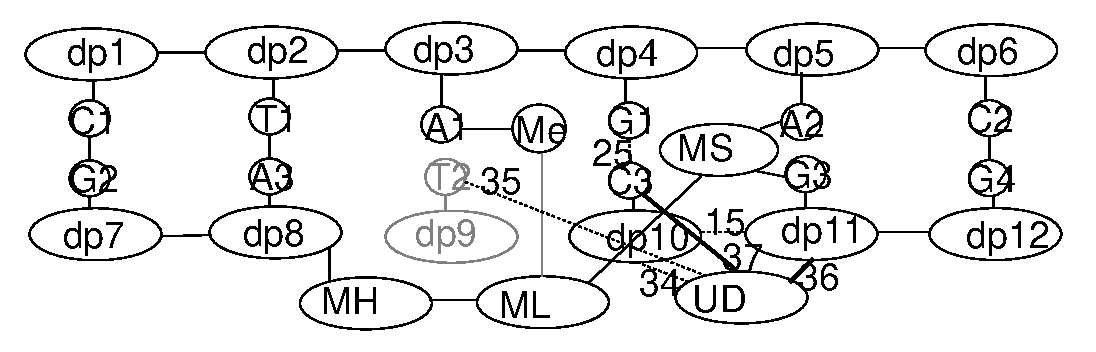
\includegraphics[width=1.0\textwidth]{mmr/state4}
  \caption[A six base pair DNA fragment.]{A six base pair DNA fragment, with a DNA mismatch and methylation of one strand. UvrD has now bonded to $C_2$ and $DP_{10}$, breaking the bonds of those molecules to the rest of the DNA via concerted actions (shown as dotted lines). This process can conitine for more pairs.}
  \label{fig:state4}
\end{figure}

This process can continue until the offending base has been removed. Figure~\ref{fig:state6} shows the removal of the offending base. We do not model how the number of base pairs to remove is determined. In reality, that number is not fixed, but is determined by the interal workings of the protein, where the number is statistically distributed. Once this is done and the MutH, MutL, and MutS proteins have detached we get the situation shown in Figure~\ref{fig:state7}. This is now ready for other proteins to replace the bases and and deoxyribose/phosphate groups. Notice that the remaining strand contains the necessary information for this, in particular only a T base can be put in opposite the A base. Note that the methyl group stays attached to $A_1$, since it is still an old DNA strand. Also the appropriate groups in the new, lower half will be methylated, so that both strands are marked as old material after the next DNA duplication process.

The modelling done so far does not involve any spatial configurataions. As in the BER example, this means that UvrD could bond to any deoxyribose/phosphate group, not just the neighbouring one. It also means that we have not modelled the formation of the loop in the DNA, which is crucial for cleaving the correct strand.

\begin{figure}[h!]
\psfrag{dp1}{${DP_1}$}
\psfrag{dp2}{${DP_2}$}
\psfrag{dp3}{${DP_3}$}
\psfrag{dp4}{${DP_4}$}
\psfrag{dp5}{${DP_5}$}
\psfrag{dp6}{${DP_6}$}
\psfrag{dp7}{${DP_7}$}
\psfrag{dp8}{${DP_8}$}
\psfrag{dp9}{${DP_9}$}
\psfrag{dp10}{${DP_{10}}$}
\psfrag{dp11}{${DP_{11}}$}
\psfrag{dp12}{${DP_{12}}$}
\psfrag{A1}[cc][][0.8][0]{${A_1}$}
\psfrag{A2}[cc][][0.8][0]{${A_2}$}
\psfrag{A3}[cc][][0.8][0]{${A_3}$}
\psfrag{T1}[cc][][0.8][0]{${T_1}$}
\psfrag{T2}[cc][][0.8][0]{${T_2}$}
\psfrag{C1}[cc][][0.8][0]{${C_1}$}
\psfrag{C2}[cc][][0.8][0]{${C_2}$}
\psfrag{C3}[cc][][0.8][0]{${C_3}$}
\psfrag{G1}[cc][][0.8][0]{${G_1}$}
\psfrag{G2}[cc][][0.8][0]{${G_2}$}
\psfrag{G3}[cc][][0.8][0]{${G_3}$}
\psfrag{G4}[cc][][0.8][0]{${G_4}$}
\psfrag{Me}{${\mathit{Me}}$}
\psfrag{MS}{${\mathit{MutS}}$}
\psfrag{ML}{${\mathit{MutL}}$}
\psfrag{MH}{${\mathit{MutH}}$}
\psfrag{UD}{${\mathit{UvrD}}$}
  \centering
    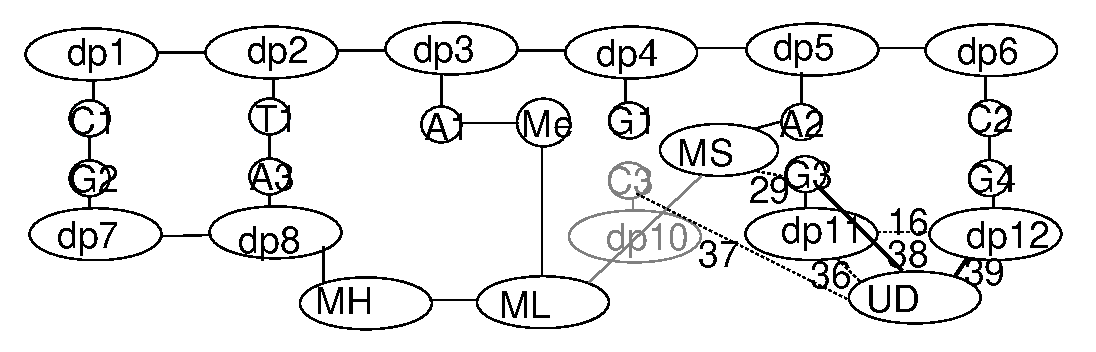
\includegraphics[width=1.0\textwidth]{mmr/state6}
  \caption[A six base pair DNA fragment.]{A six base pair DNA fragment, with a DNA mismatch and methylation of one strand. UvrD has now bonded to $G_3$ (the offendingn base) and $DP_{11}$, breaking the bonds of those molecules to the rest of the DNA via concerted actions (shown as dotted lines). The offending base is removed after this step.}
  \label{fig:state6}
\end{figure}

\begin{figure}[h!]
\psfrag{dp1}{${DP_1}$}
\psfrag{dp2}{${DP_2}$}
\psfrag{dp3}{${DP_3}$}
\psfrag{dp4}{${DP_4}$}
\psfrag{dp5}{${DP_5}$}
\psfrag{dp6}{${DP_6}$}
\psfrag{dp7}{${DP_7}$}
\psfrag{dp8}{${DP_8}$}
\psfrag{dp9}{${DP_9}$}
\psfrag{dp10}{${DP_{10}}$}
\psfrag{dp11}{${DP_{11}}$}
\psfrag{dp12}{${DP_{12}}$}
\psfrag{A1}[cc][][0.8][0]{${A_1}$}
\psfrag{A2}[cc][][0.8][0]{${A_2}$}
\psfrag{A3}[cc][][0.8][0]{${A_3}$}
\psfrag{T1}[cc][][0.8][0]{${T_1}$}
\psfrag{T2}[cc][][0.8][0]{${T_2}$}
\psfrag{C1}[cc][][0.8][0]{${C_1}$}
\psfrag{C2}[cc][][0.8][0]{${C_2}$}
\psfrag{C3}[cc][][0.8][0]{${C_3}$}
\psfrag{G1}[cc][][0.8][0]{${G_1}$}
\psfrag{G2}[cc][][0.8][0]{${G_2}$}
\psfrag{G3}[cc][][0.8][0]{${G_3}$}
\psfrag{G4}[cc][][0.8][0]{${G_4}$}
\psfrag{Me}{${\mathit{Me}}$}
\psfrag{MS}{${\mathit{MutS}}$}
\psfrag{ML}{${\mathit{MutL}}$}
\psfrag{MH}{${\mathit{MutH}}$}
\psfrag{UD}{${\mathit{UvrD}}$}
  \centering
    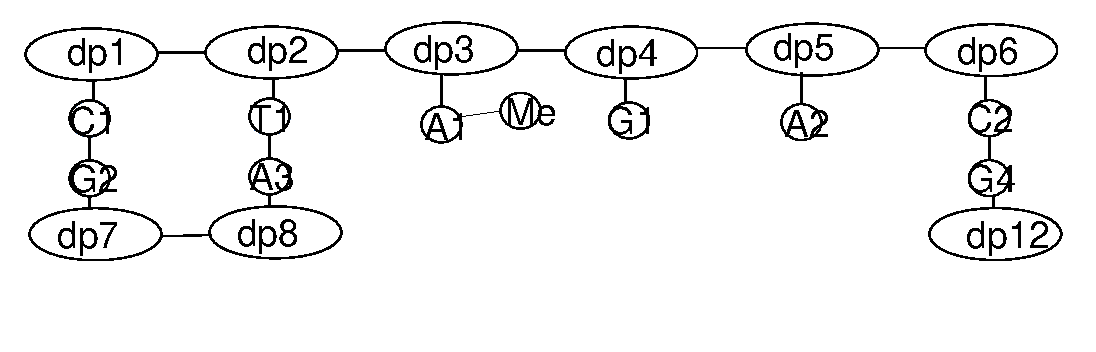
\includegraphics[width=1.0\textwidth]{mmr/state7}
  \caption[A six base pair DNA fragment.]{A six base pair DNA fragment, with a gap in one strand produced by MMR. This is now ready to replaced with correct information.}
  \label{fig:state7}
\end{figure}


